\documentclass[10pt,a4paper]{article}
\usepackage[utf8]{inputenc}
\usepackage{amsmath}
\usepackage{amsfonts}
\usepackage{amssymb}
\usepackage{listings}
\usepackage{graphicx}
\lstset{showstringspaces=false,
		breaklines=true,
		postbreak=\raisebox{0ex}[0ex][0ex]{\ensuremath{\hookrightarrow\space}}}
    	
\begin{document}
\title{Intelligent Systems Assignment 2}
\author{Wessel Becker (1982362) \& Sander ten Hoor (2318555)}
\maketitle

\section{Matlab Code}
The following code was created to obtain the plots.

\subsection{main.m}
\lstinputlisting[language=Matlab]{./VQ/main.m}

\subsection{changeDistance.m}
\lstinputlisting[language=Matlab]{./VQ/changeDistance.m}

\subsection{randomDataPoints.m}
\lstinputlisting[language=Matlab]{./VQ/randomDataPoints.m}

\subsection{vectorQuantization.m}
\lstinputlisting[language=Matlab]{./VQ/vectorQuantization.m}

\subsection{euclidean.m}
\lstinputlisting[language=Matlab]{./VQ/euclidean.m}

\subsection{vectorQuantization.m}
\lstinputlisting[language=Matlab]{./VQ/vectorQuantization.m}	

\subsection{quantizationError.m}
\lstinputlisting[language=Matlab]{./VQ/quantizationError.m}

\subsection{plotVQ.m}
\lstinputlisting[language=Matlab]{./VQ/plotVQ.m}

\subsection{plotLearningCurve.m}
\lstinputlisting[language=Matlab]{./VQ/plotLearningCurve.m}

\section{Plots}
For plotting, dataset x was chosen. The values for the learning rate were 0.1, 0.01, 0.001, 0.004. ??

\makebox[\textwidth]{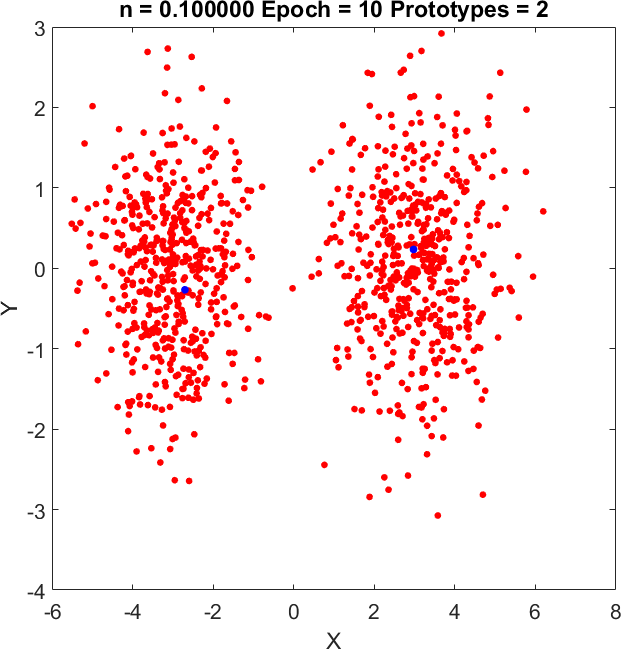
\includegraphics[width=\textwidth]{./VQ/x_e10_n01_k2}} \\

\makebox[\textwidth]{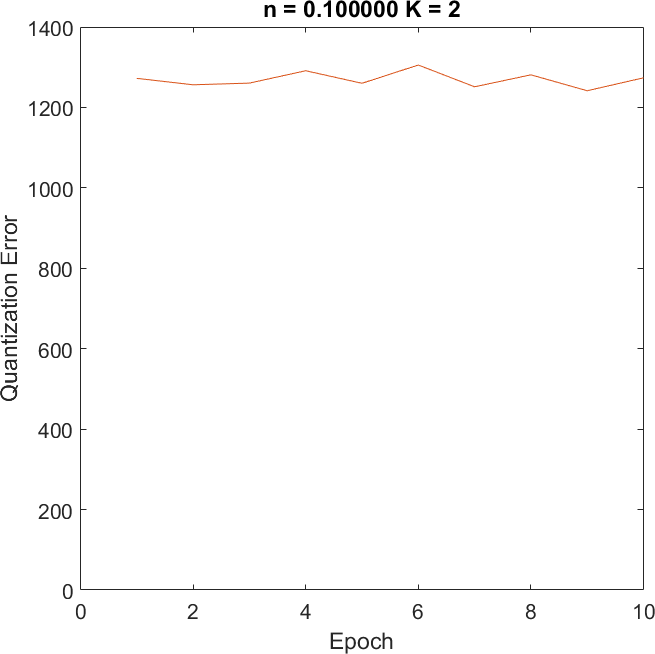
\includegraphics[width=\textwidth]{./VQ/x_e10_n01_k2_learning}} \\

\makebox[\textwidth]{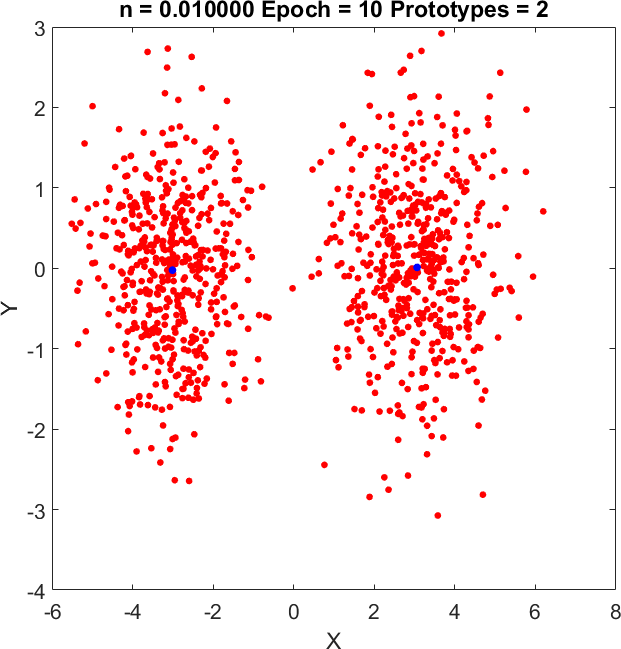
\includegraphics[width=\textwidth]{./VQ/x_e10_n001_k2}} \\

\makebox[\textwidth]{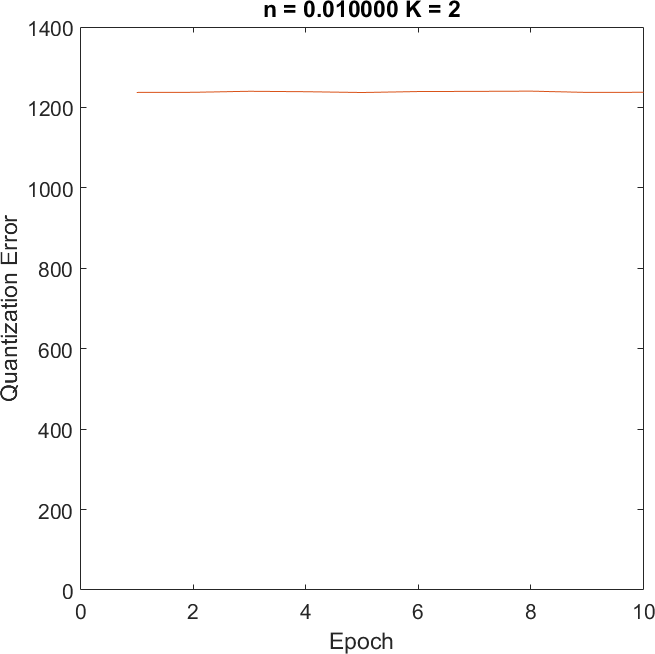
\includegraphics[width=\textwidth]{./VQ/x_e10_n001_k2_learning}} \\

\makebox[\textwidth]{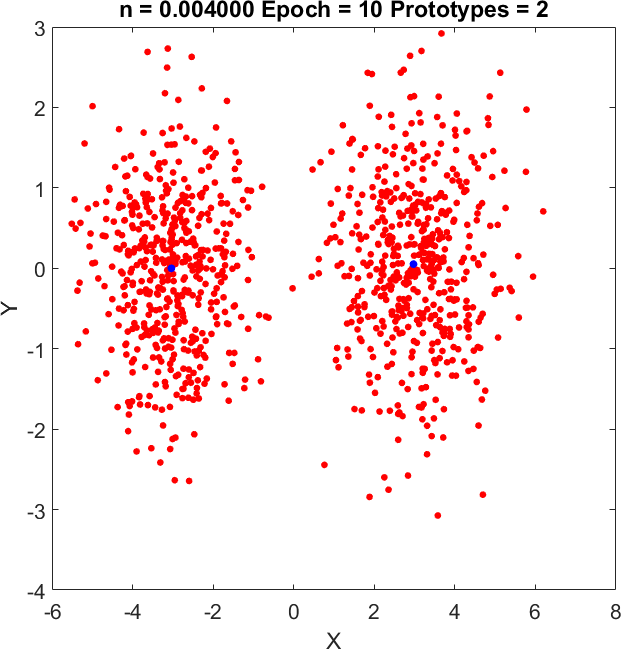
\includegraphics[width=\textwidth]{./VQ/x_e10_n0004_k2}} \\

\makebox[\textwidth]{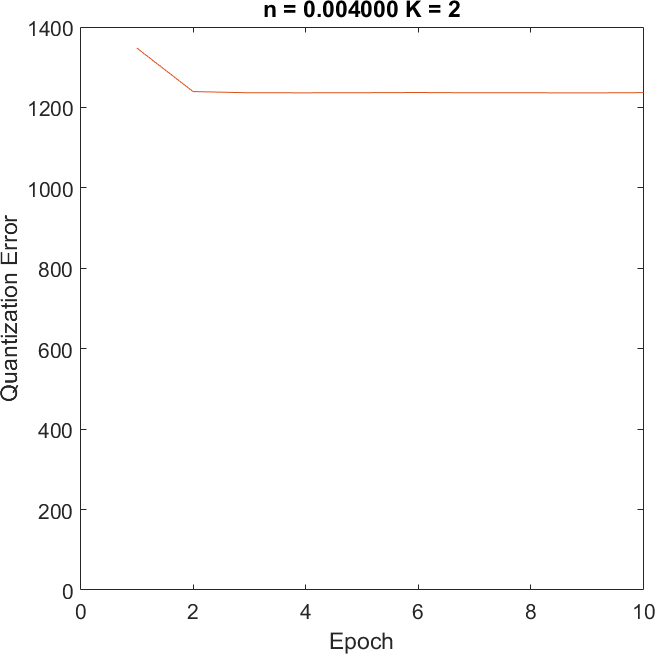
\includegraphics[width=\textwidth]{./VQ/x_e10_n0004_k2_learning}} \\

\makebox[\textwidth]{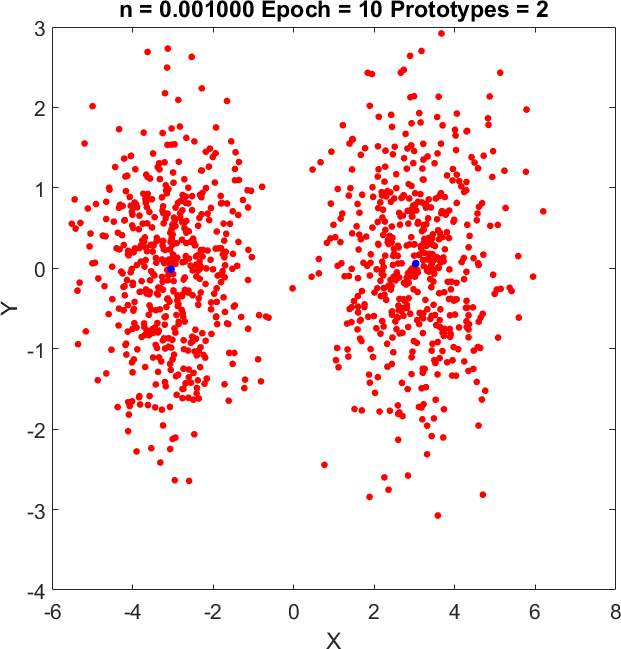
\includegraphics[width=\textwidth]{./VQ/x_e10_n0001_k2}} \\

\makebox[\textwidth]{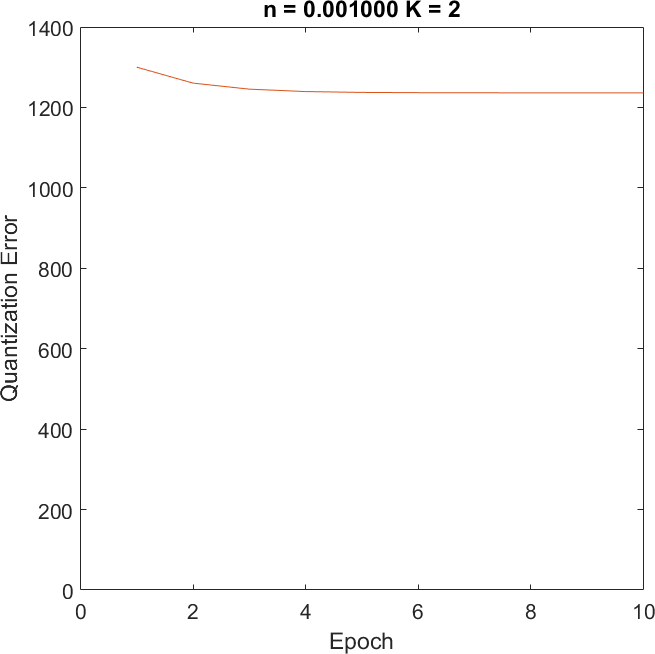
\includegraphics[width=\textwidth]{./VQ/x_e10_n0001_k2_learning}} \\

\makebox[\textwidth]{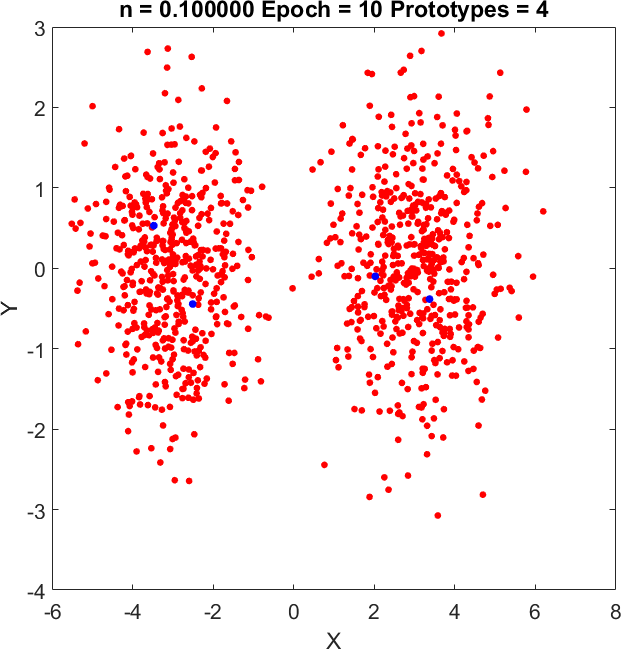
\includegraphics[width=\textwidth]{./VQ/x_e10_n01_k4}} \\

\makebox[\textwidth]{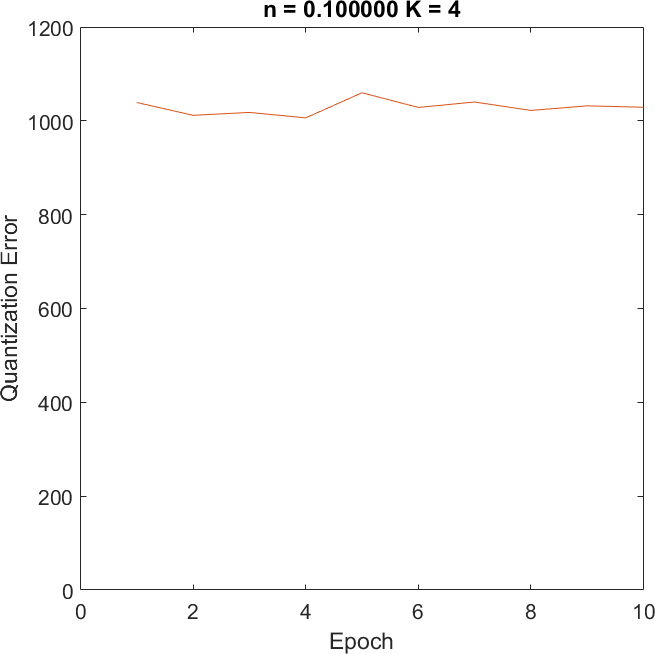
\includegraphics[width=\textwidth]{./VQ/x_e10_n01_k4_learning}} \\

\makebox[\textwidth]{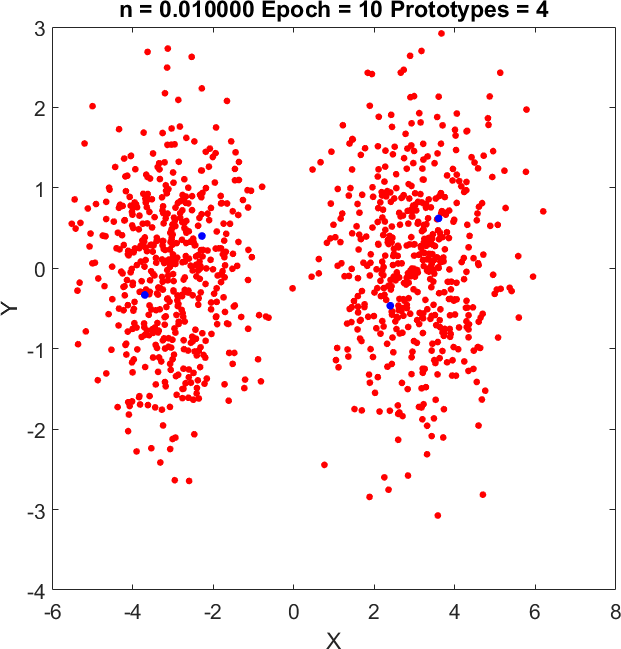
\includegraphics[width=\textwidth]{./VQ/x_e10_n001_k4}} \\

\makebox[\textwidth]{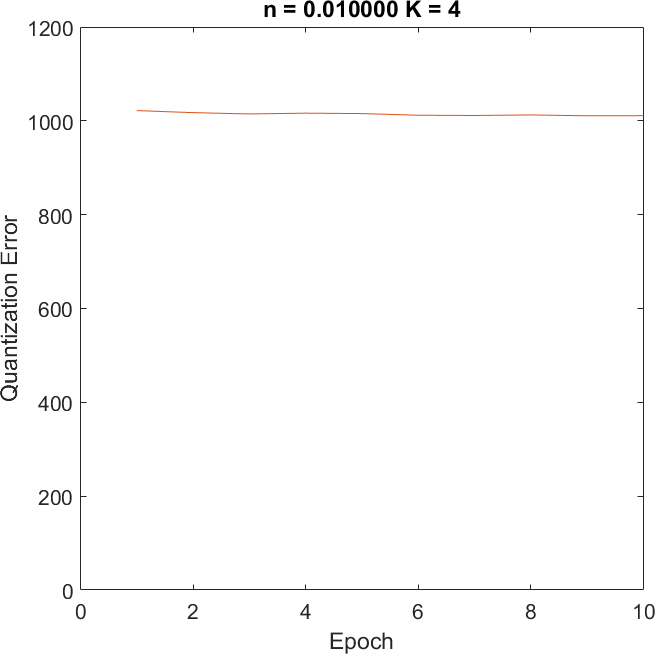
\includegraphics[width=\textwidth]{./VQ/x_e10_n001_k4_learning}} \\

\makebox[\textwidth]{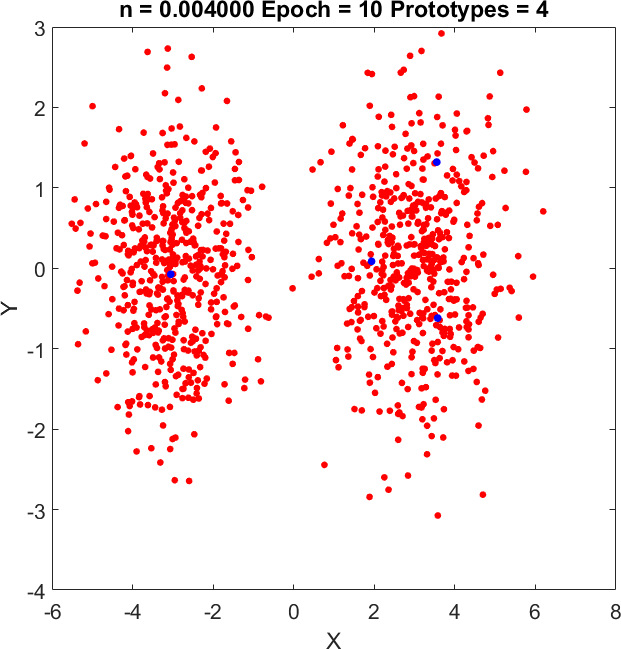
\includegraphics[width=\textwidth]{./VQ/x_e10_n0004_k4}} \\

\makebox[\textwidth]{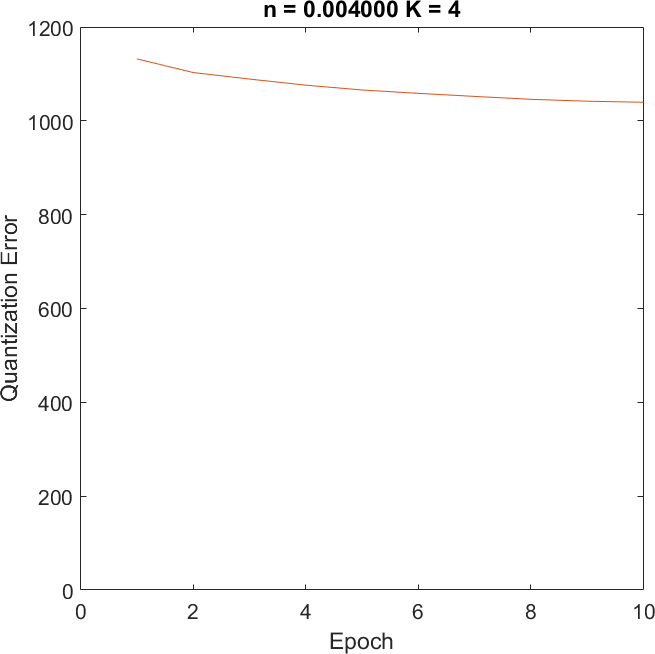
\includegraphics[width=\textwidth]{./VQ/x_e10_n0004_k4_learning}} \\

\makebox[\textwidth]{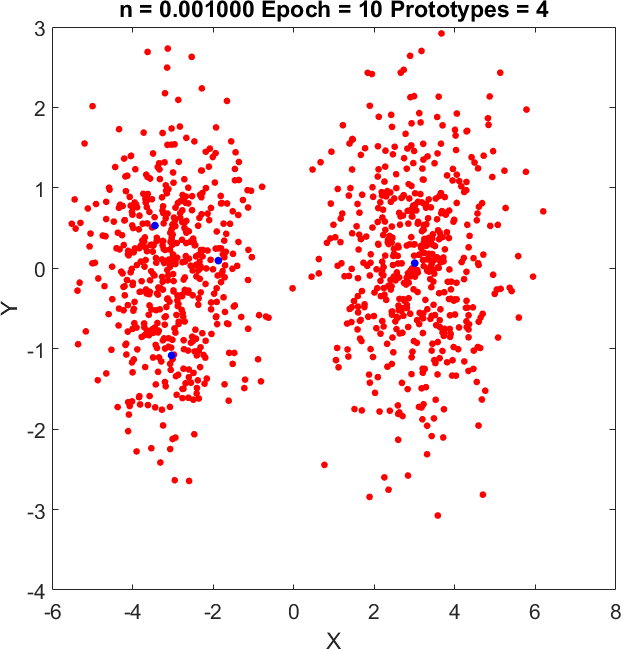
\includegraphics[width=\textwidth]{./VQ/x_e10_n0001_k4}} \\

\makebox[\textwidth]{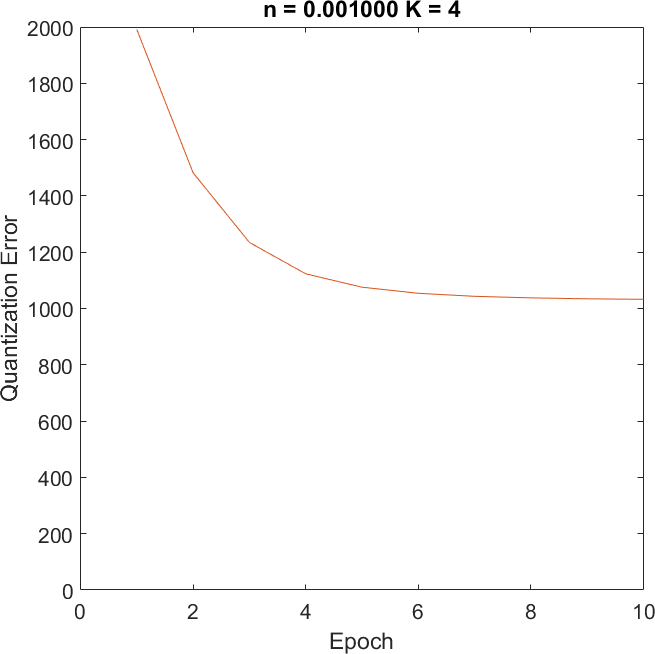
\includegraphics[width=\textwidth]{./VQ/x_e10_n0001_k4_learning}} \\

\section{Discussion}
At higher learning rates, the quantization error does not seem to clearly improve over time. This could be the result of large movements accross the datapoints, or the local minimum is reached quickly. By lowering the learning rate, the quantization errors becomes more constant at first, and then start dropping. However, they all become relatively constant after only a few epochs except for one. 

\subsection{Fluctuation}
At higher learning rates, the quantization error fluctuates a lot more than at lower learning rates, where the graph becomes smoother.

\subsection{Number of prototypes}
When the number of prototypes is higher, the learning process goes slower. This is because everytime the distance is evaluated, still only one prototype is updated. If the number of prototypes is twice as large as before, the learning speed is cut in half.

\subsection{Winner takes all}
In one of the plots, there are three prototypes in one half, and one in the other. This affects the quantization error, which would be lower if there were two prototypes on each side. However, this state is achieved because only the winner is updated. In the right half, the winner is always the sole prototype there.

\section{Work done}
For this assignment, the algorithm implementation was done by Wessel, while Sander worked on plotting. The latter created the plots and put together this document, after which Wessel made some suggestions and modifications.

\end{document}